\chapter{Débits classés}

\section{Explication}
\begin{itemize}
    \item On fait du classement de débits pour pouvoir calculer un débit d'étiage.
    \item Calculer un débit d'étiage est utile pour connaître le volume maximal à préveler dans un cours d'eau
\end{itemize}

\section{Divers schémas}
\begin{figure}[H]
    \centering
    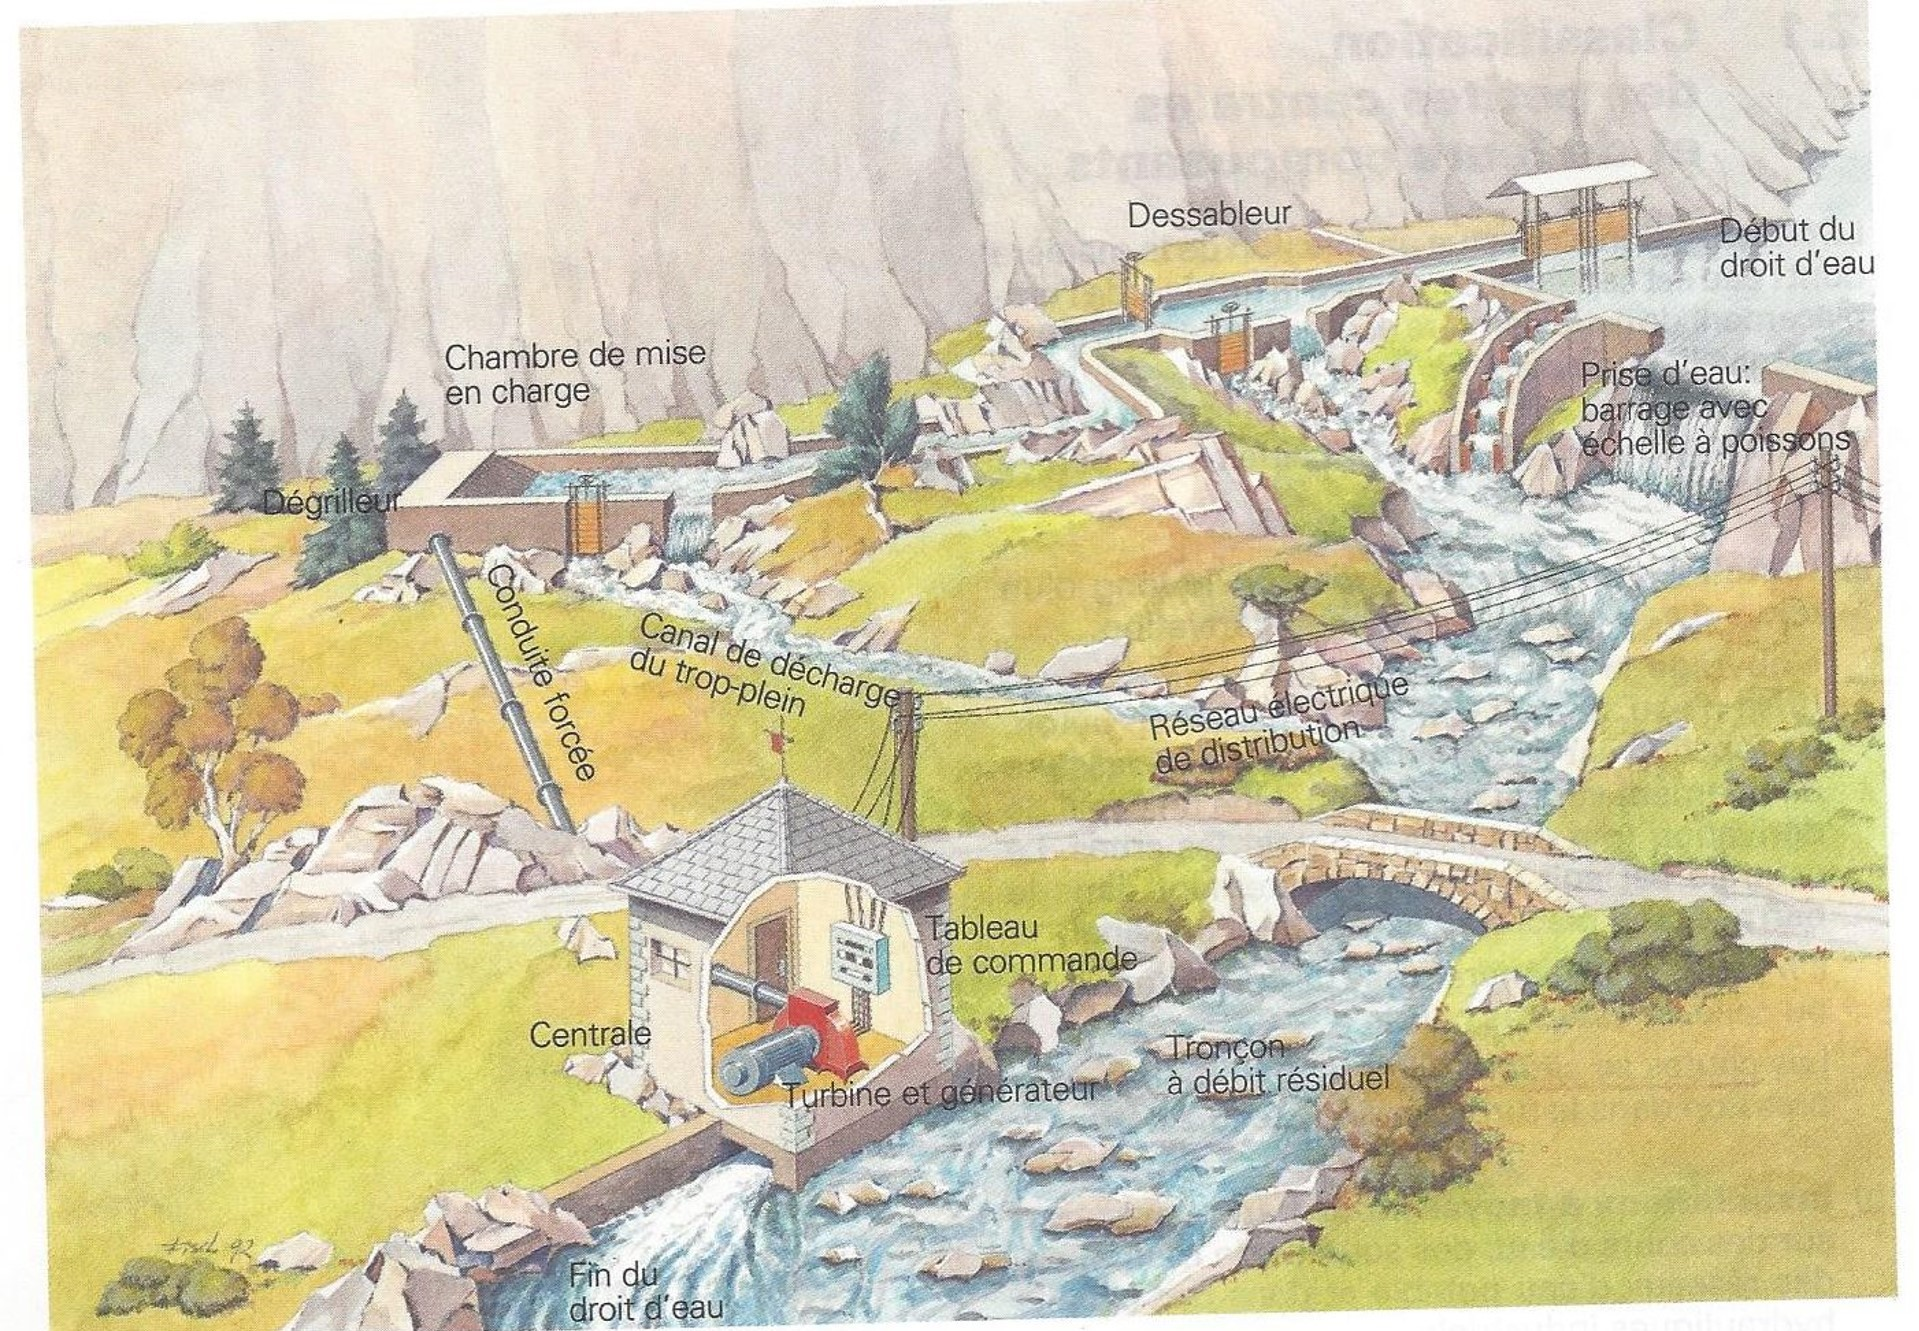
\includegraphics[width=15cm]{photoCentraleEnergieElectrique.jpg}
    \caption{Vue d'ensemble d'une centrale à haute pression sur canal de dérivation}
\end{figure}

\begin{figure}[H]
    \centering
    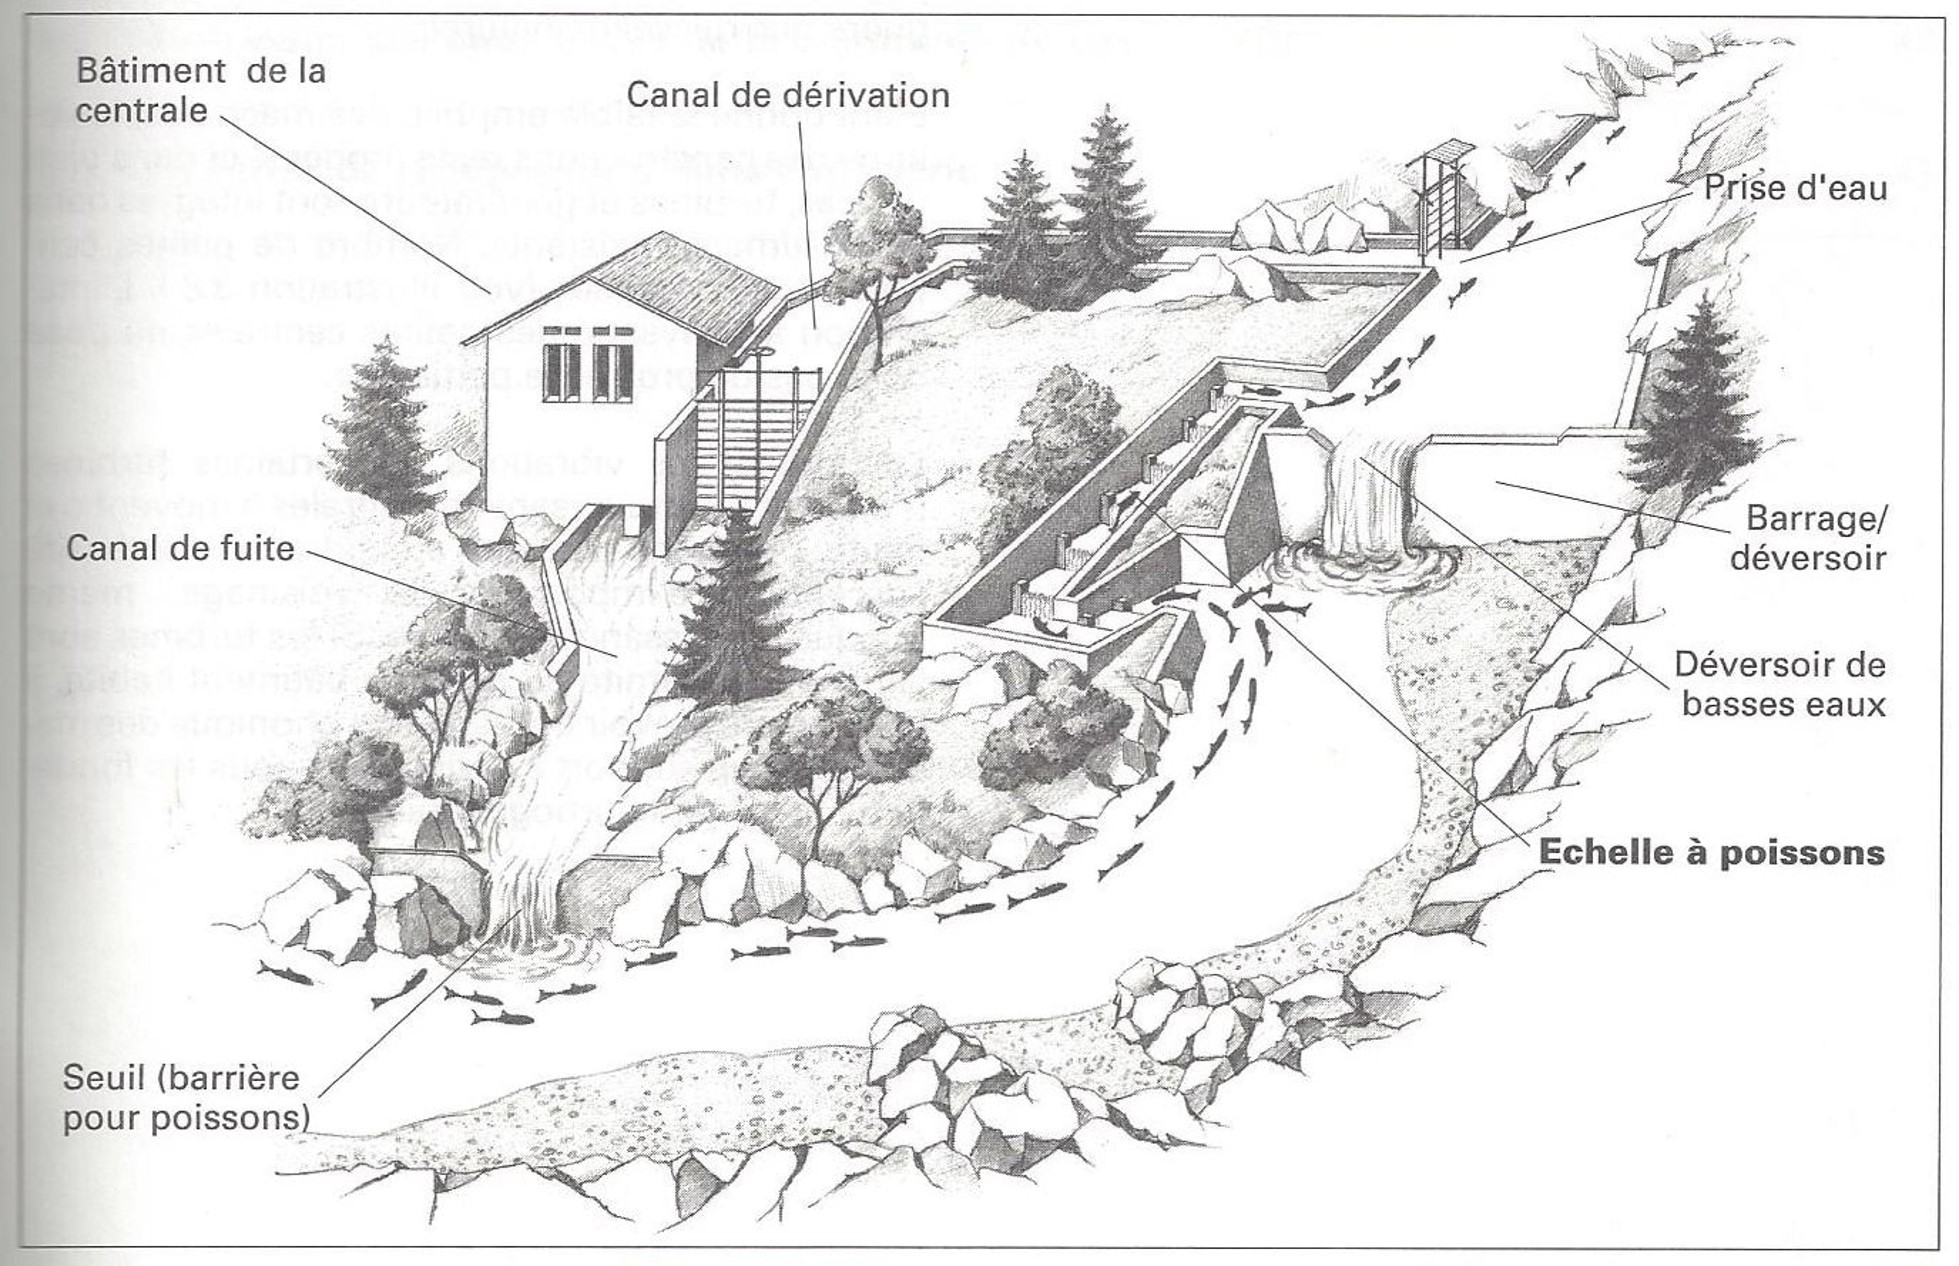
\includegraphics[width=15cm]{schemaPriseEauPassePoisson.jpg}
    \caption{Schéma d'une prise d'eau avec passe à poisson}
\end{figure}

\begin{figure}[H]
    \centering
    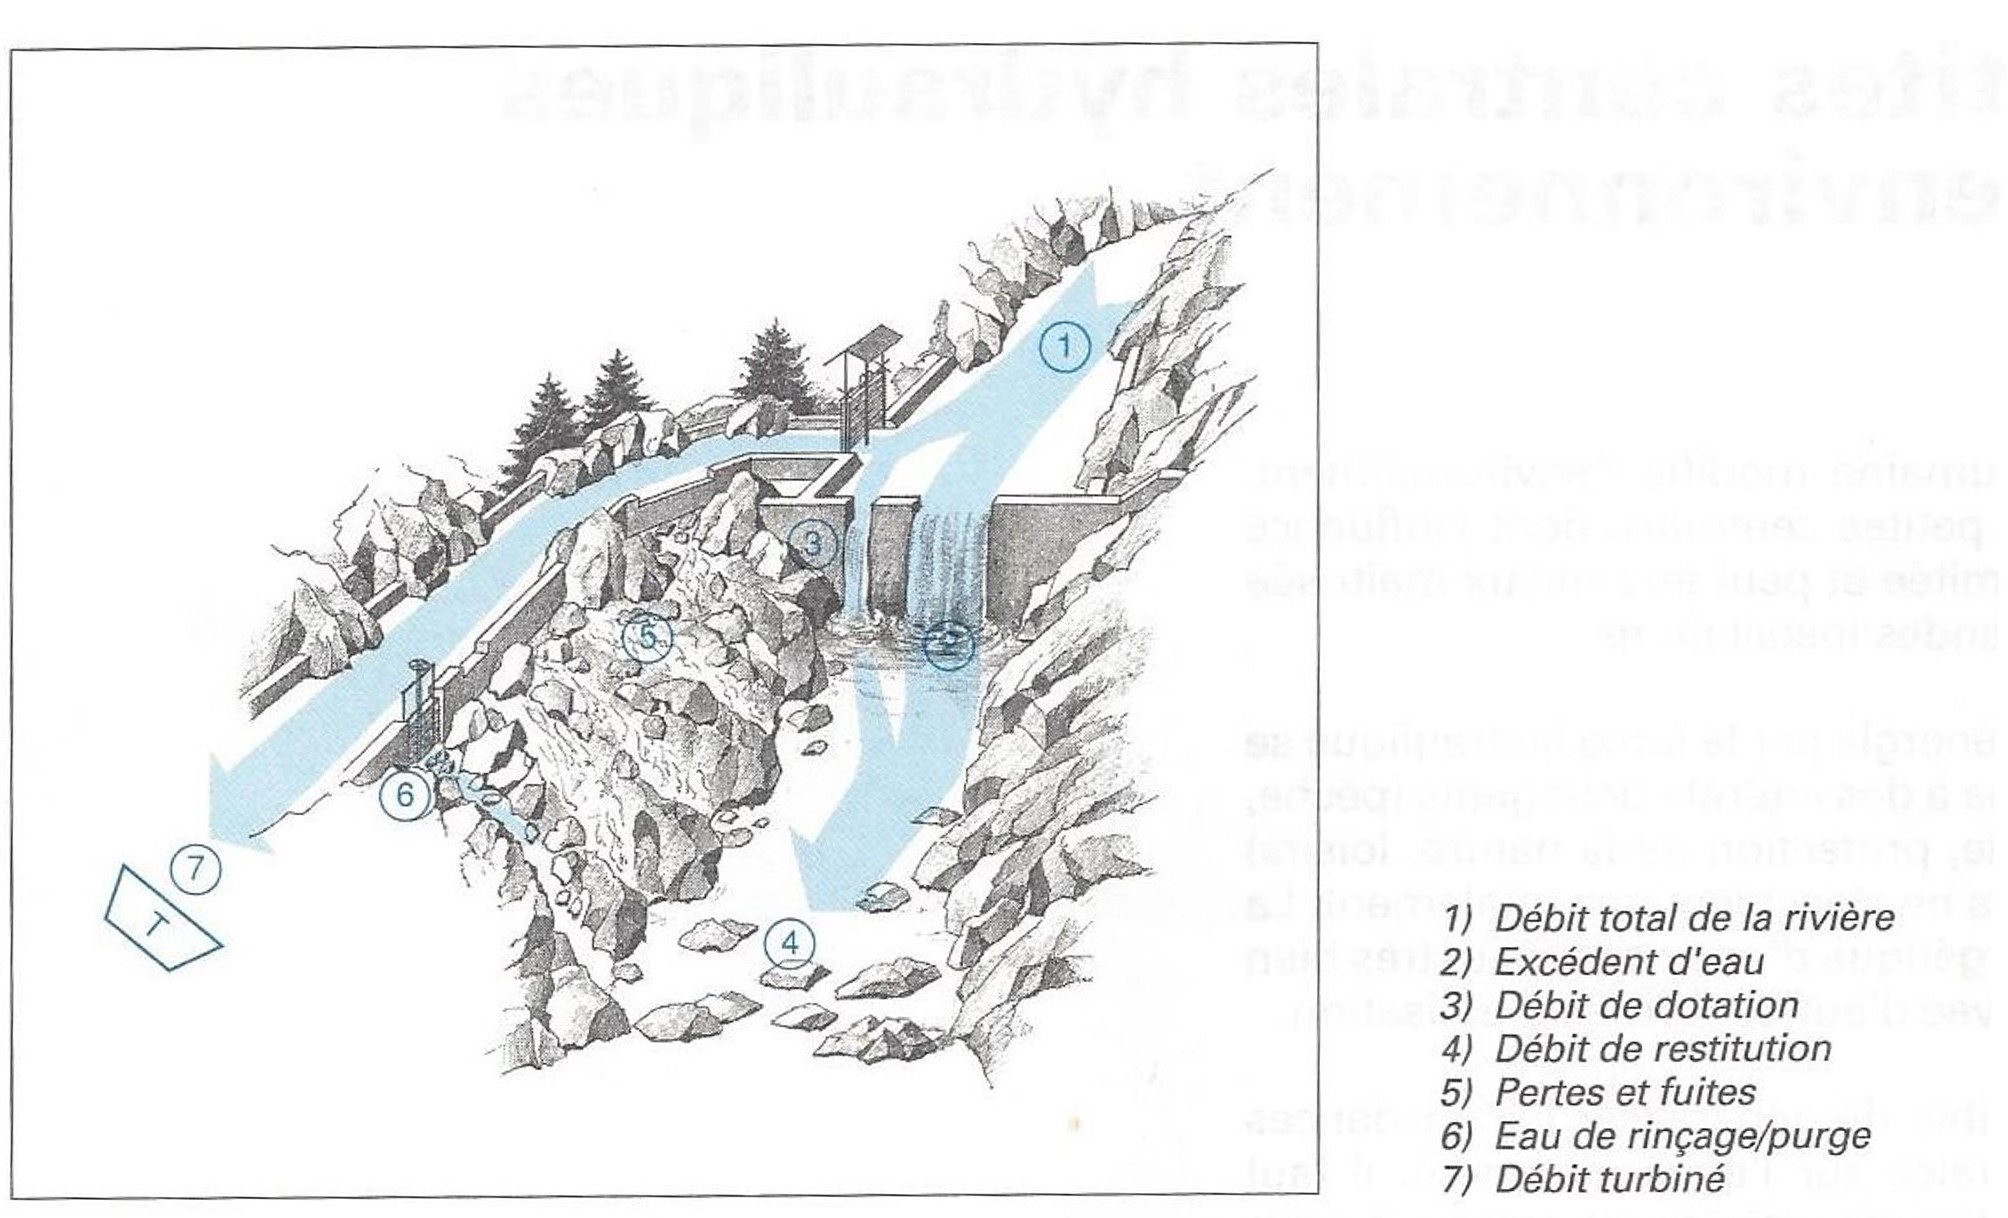
\includegraphics[width=15cm]{schemaDefinition.jpg}
    \caption{Définition de plusieurs termes}
\end{figure}

\begin{figure}[H]
    \centering
    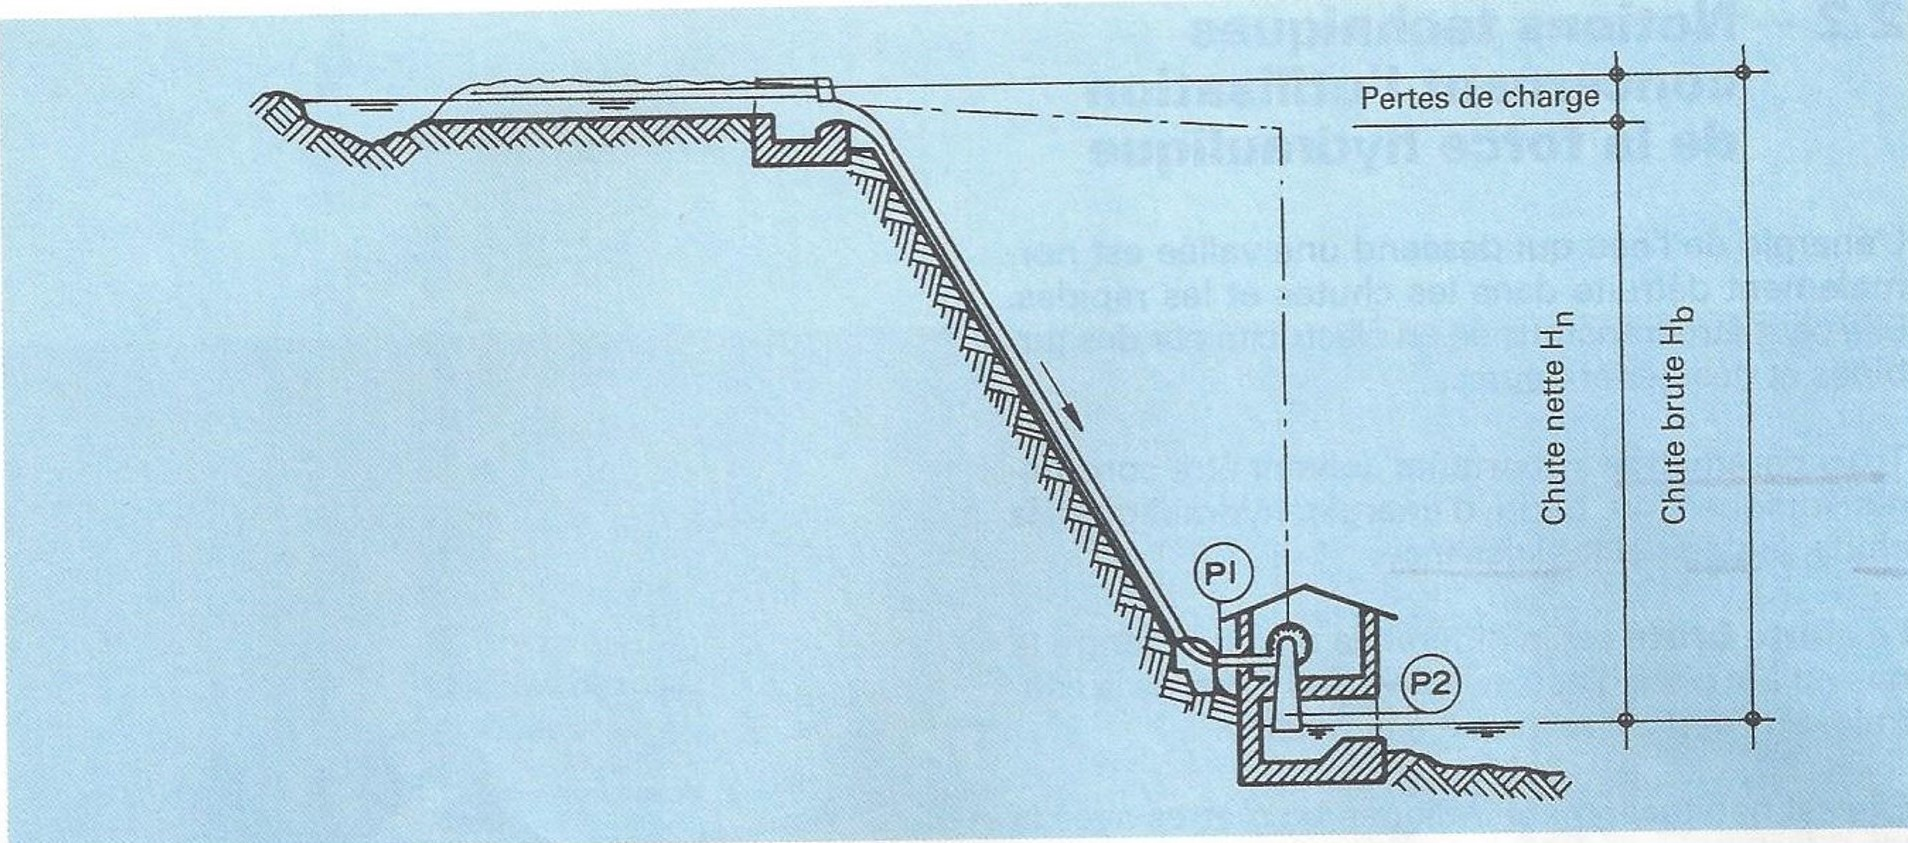
\includegraphics[width=15cm]{schemaPriseEau.jpg}
    \caption{Paramètre hydraulique d'une prise d'eau avec hauteur de chute réelle et effective}
\end{figure}

\begin{figure}[H]
    \centering
    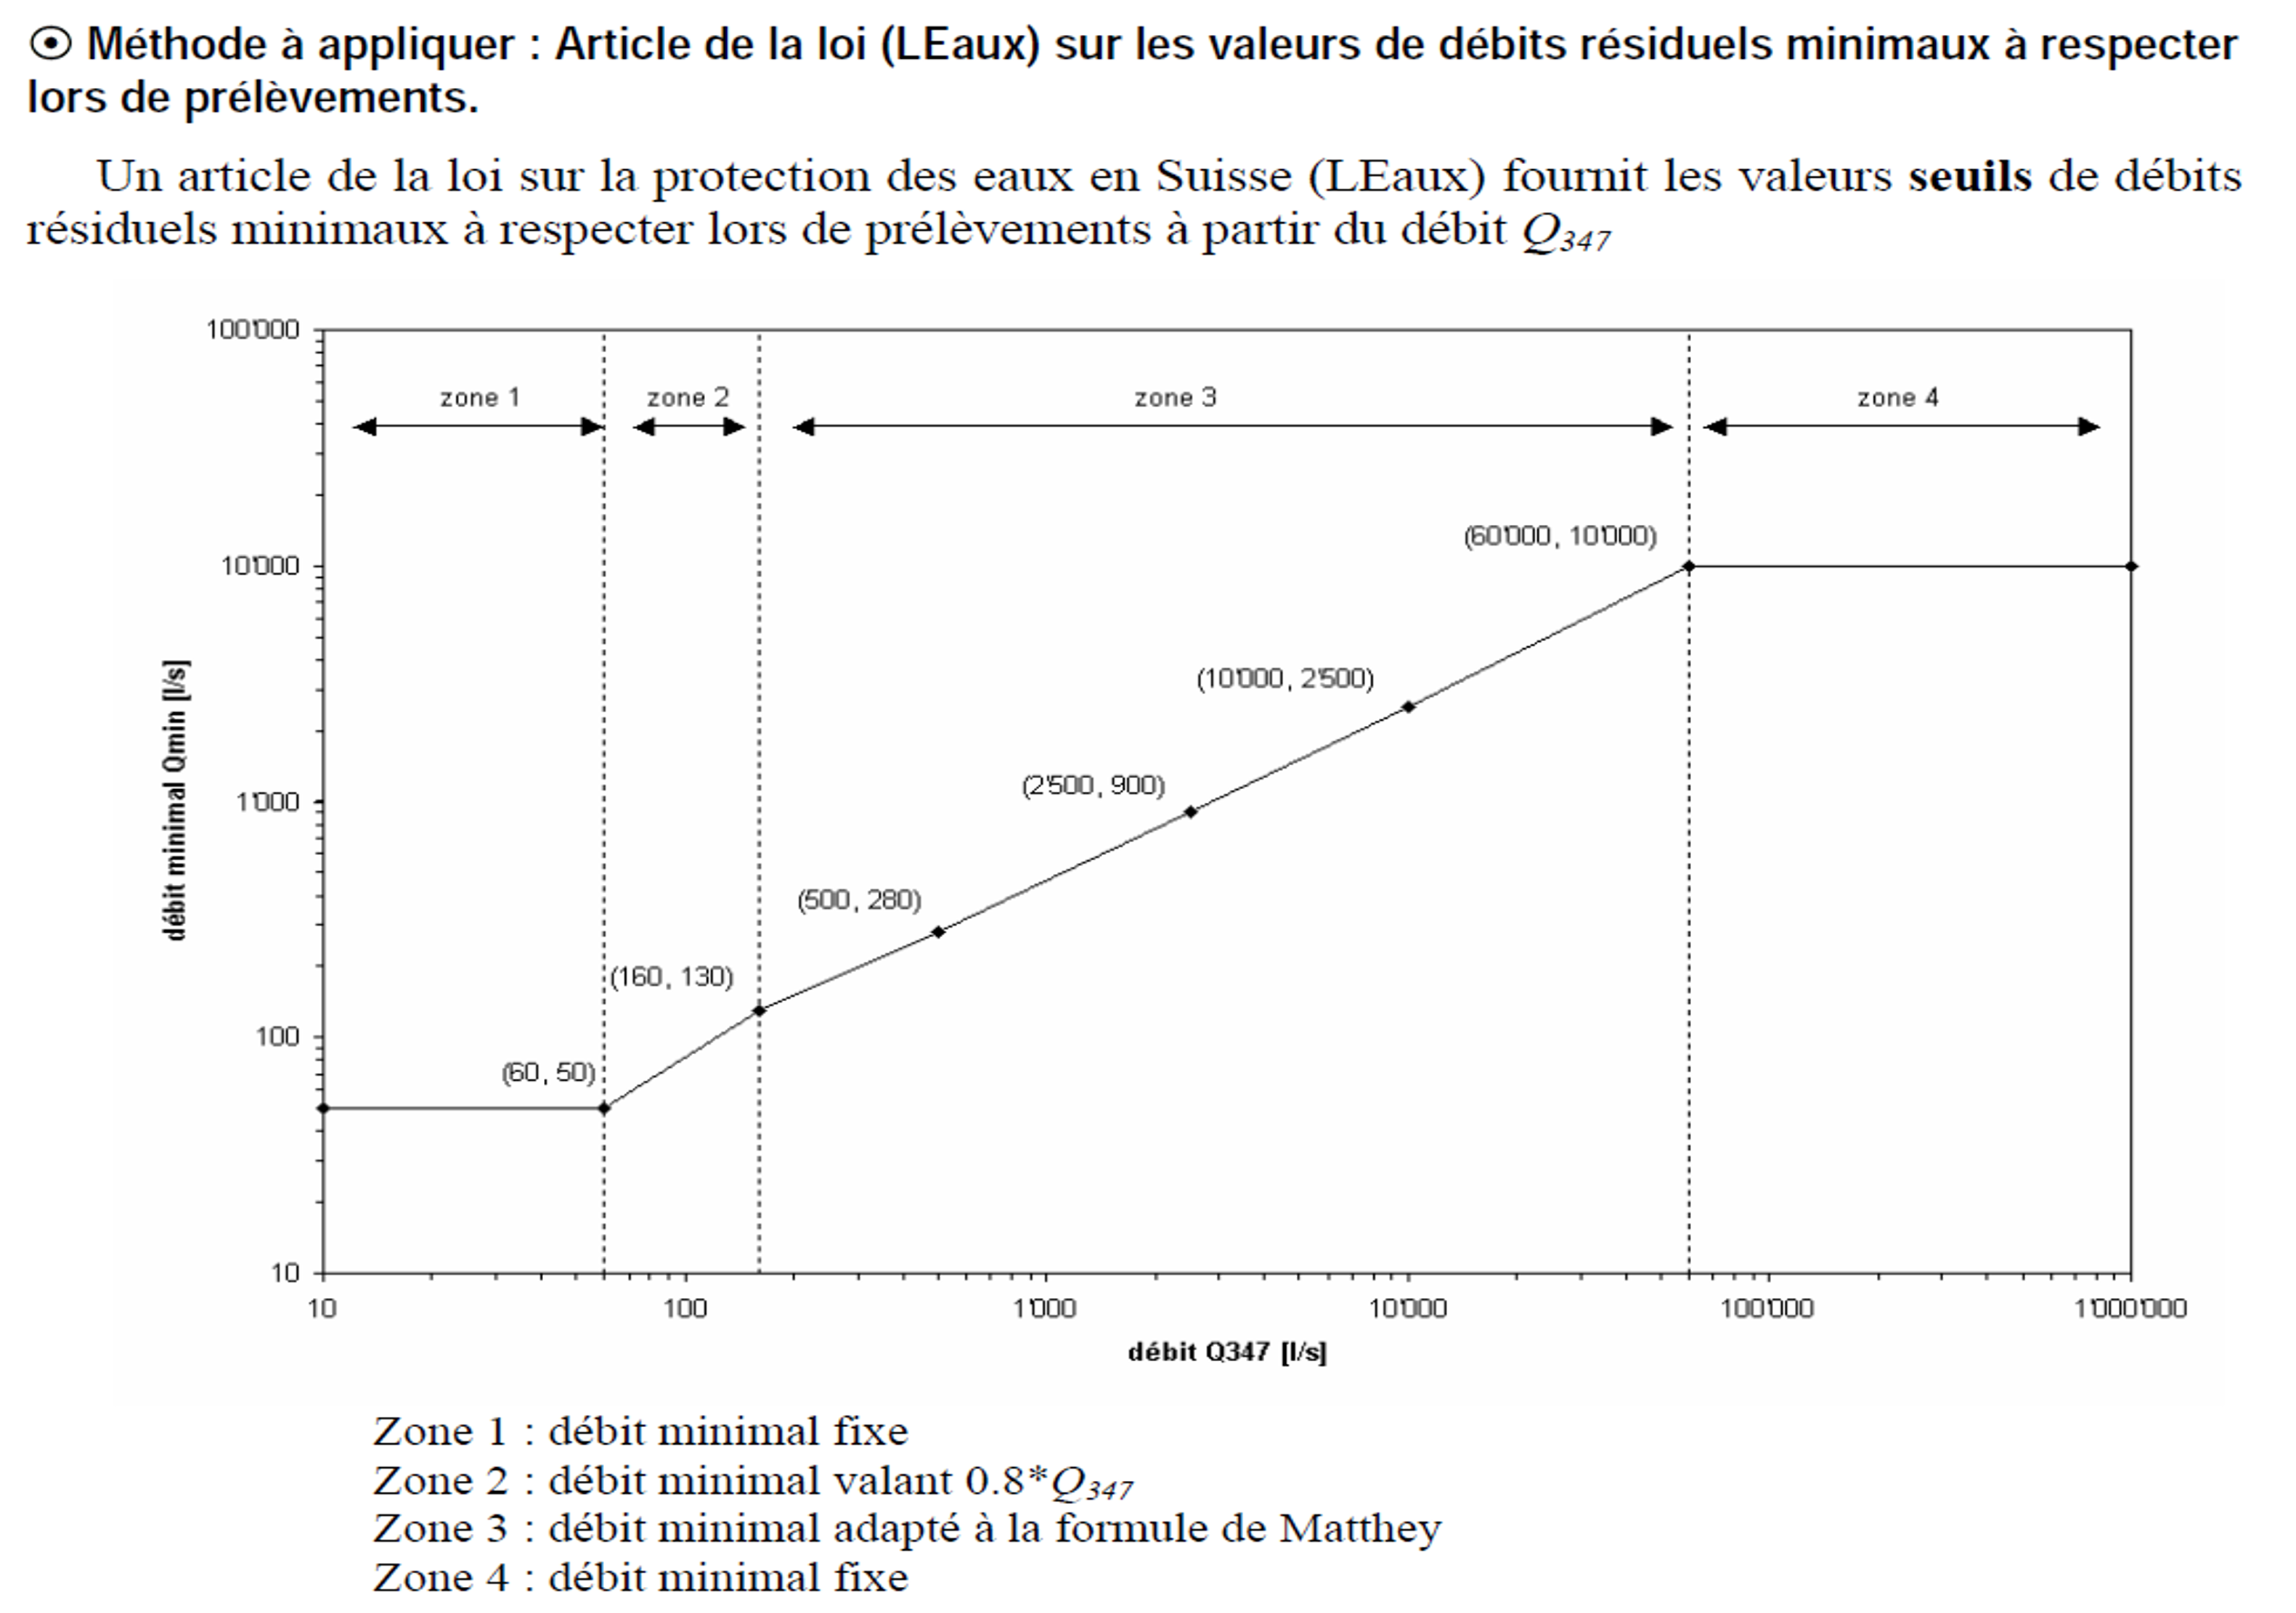
\includegraphics[width=15cm]{loiDebitQ347.png}
    \caption{Loi suisse sur les débits minimaux et utilisation du Q347}
    \label{fig:loiQ347}
\end{figure}


\section{Méthode statistique}
\begin{itemize}
    \item Il faut des valeurs journalières
    \item Série de données de 10 ans moins
    \item On classe les débits du plus petit au plus grands
    \item cf. Annexe \ref{chap:courbeClasses}
\end{itemize}

\section{Régimes hydrologiques}
\begin{itemize}
    \item Un régime hydrologique décrit les variations mensuelles des 12 débits moyens mensuels
    \item Cela représente un intérêt pour déterminer le Q347 qui selon la législation doit correspondre à un régime naturel du cours d'eau et pas influencé par des ouvrages d'hydrauliques, captages, barrages, prises d'eau, etc.
\end{itemize}

\subsection{Coefficients de Pardé (Pki)}
\begin{figure}[H]
    \centering
    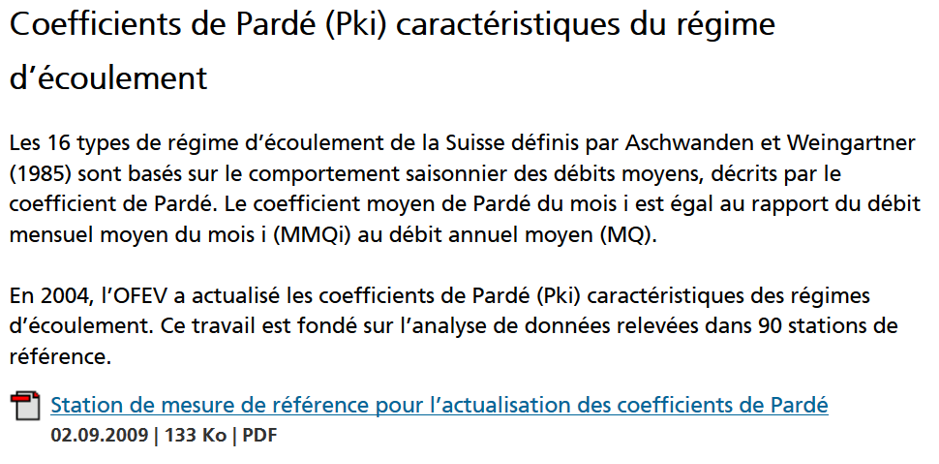
\includegraphics[width=15cm]{coefficientParde.png}
\end{figure}
Pour calculer des coefficients de Pardé :
\begin{enumerate}
    \item Débit annuel moyen sur plusieurs années
    \item Calcul du débit moyen mensuel pour chacun des 12 mois de l'année
    \item Pour chaque mois de l'année, on calcule le rapport entre le débit moyen de chaque mois et le débit moyen annuels.
    \item Les 12 rapports sont les 12 coefficients de Pardé.
\end{enumerate}

\subsection{Détermination d'un régime}
\begin{figure}[H]
    \centering
    \subfigure[Paramètre géographique]{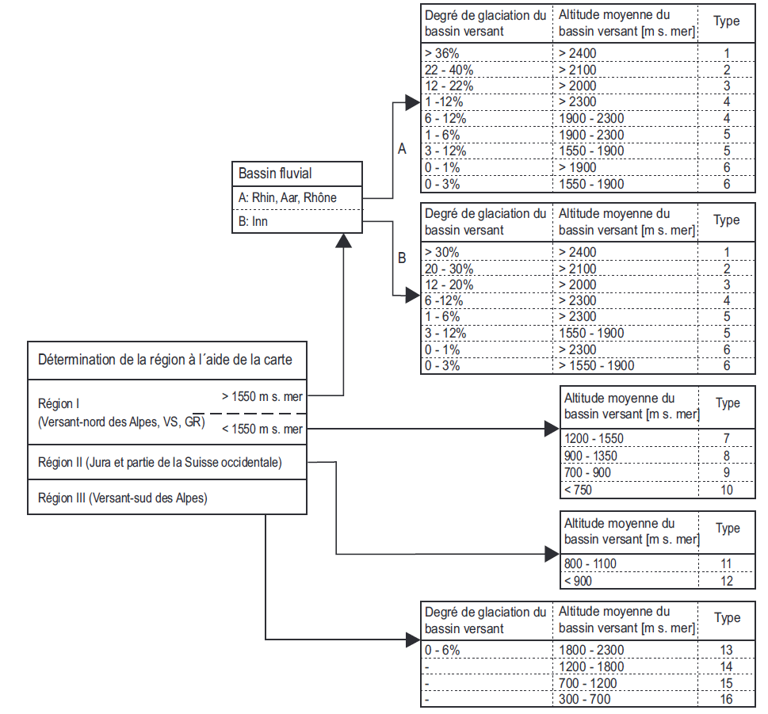
\includegraphics[width=12cm]{determinerType.png}} \\
    \subfigure[map.geo.admin.ch]{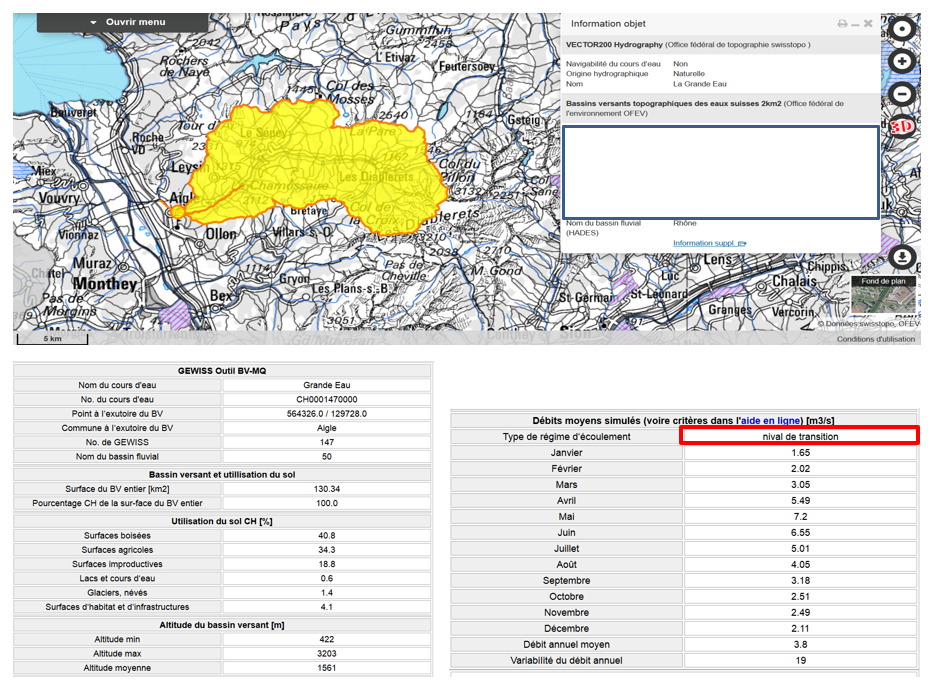
\includegraphics[width=10cm]{mapGeoAdmin.png}} \\
    \subfigure[Médiane]{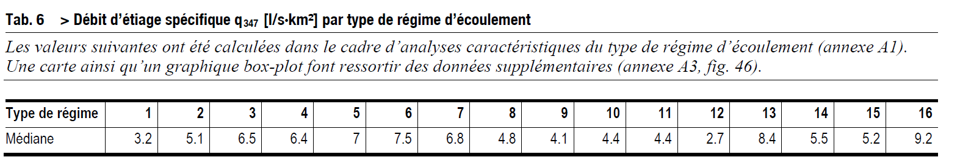
\includegraphics[width=17cm]{debitEtiageRegime.png}}
\end{figure}

\begin{figure}[H]
    \subfigure[]{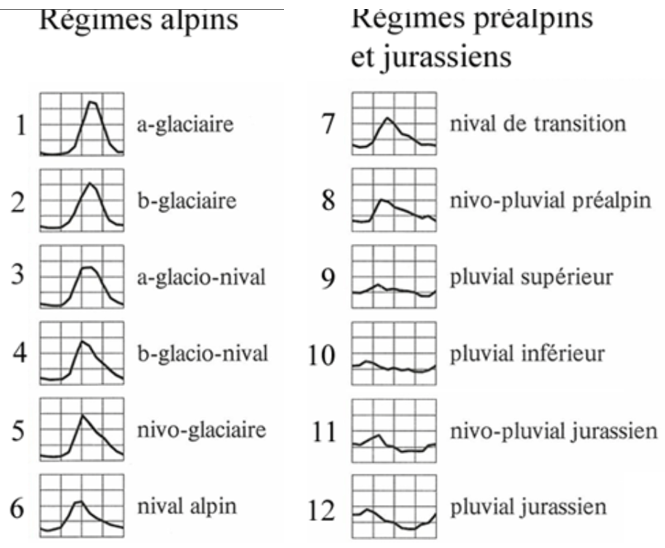
\includegraphics[width=7cm]{regimesHydro.png}} 
    \hfill
    \subfigure[]{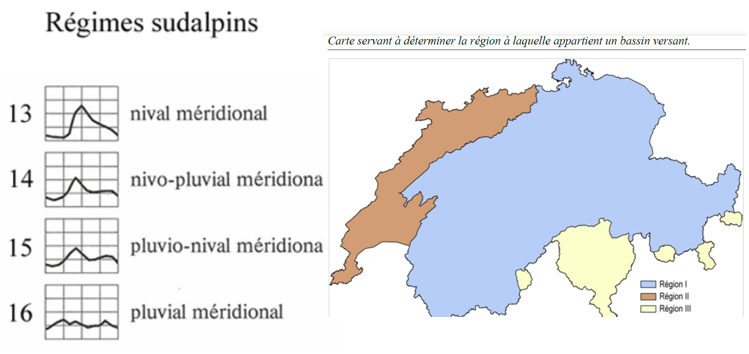
\includegraphics[width=7cm]{regimesHydro2.png}}
\end{figure}

Pour calculer un Q347 avec les informations du bassins versant, il faut simplement multiplier la suface en km\up{2} du bassin versant et le débit d'étiage du cours d'eau du régime.
\begin{equation}
    Q347 = Surface * médiane
\end{equation}

\section{Débits minimaux}
\begin{itemize}
    \item \textbf{Débit Q347 :} débit atteint ou dépassé en moyenne 347 jours par année
    \item \textbf{Débit Q300 :} débit 300 jours, dans certains pays
    \item \textbf{Débit DCE :} 10 mois, dans d'autres pays
    \item \textbf{Débit DC10 :} 355 jours, dans encore d'autre pays
\end{itemize}

\section{Exemple d'application}
\subsection{Formules}
\begin{itemize}
    \item Puissance hydraulique théorique [W] $= 1000 \cdot 9.81 \cdot Q \cdot H$
    \item Puissance hydraulique effective [W] $= \varpi \cdot \text{Puiss. hydraulique théo.}$
\end{itemize}
Avec :
\begin{itemize}
    \item $Q$ : débit en [m3/s]
    \item $H$ : hauteur de chute [m]
    \item $\varphi$ : coefficient de rendement, entre 0.6 et 0.9
\end{itemize}

\subsection{Mise en application}
\begin{figure}[H]
    \centering
    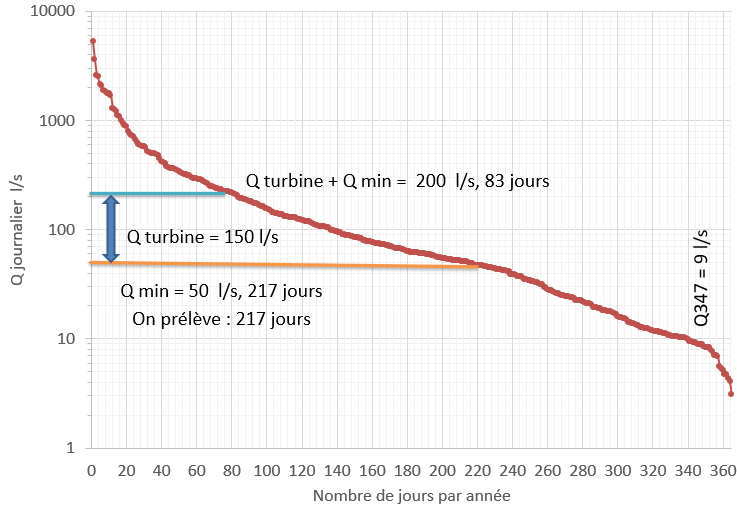
\includegraphics[width=15cm]{exempleApplication_1.png}
    \caption{Exemple d'application}
\end{figure}

\begin{itemize}
    \item Puissance hydraulique théorique [W] $= 1000 \cdot 9.81 \cdot 0.150 \cdot 100 = 147'150$
    \item Puissance hydraulique effective [W] $= 0.7 \cdot 147'150 = 103'005$
    \item Production annuelle d'énergie [kWh] $= \cfrac{1}{1000}  \cdot 103'005 \cdot 83 \cdot 24 = 205'185$
\end{itemize}